\section{Problema 4}

\subsection*{Problema 4}

\textbf{Implementa el algoritmo Spline Natural Cúbico y realiza la interpolación para la ecuación \ref{eq:problema4a} a partir de los siguientes puntos de las ecuaciones \ref{eq:x_points} y \ref{eq:y_points}.}
\begin{equation}
	f(x) = \frac{x}{1+x^2} \label{eq:problema4a}
\end{equation}

\begin{align}
	x & = \frac{i-8}{2} \qquad i=0,1,2,\dots,16 \label{eq:x_points} \\
	y & = f(x) \label{eq:y_points}
\end{align}

Las ecuación \ref{eq:x_points} fue modificada para obtener más valores en el mismo rango. La modificación esta representada en la ecuación \ref{fig:x_points_modificada}.

\begin{equation}
	x = \frac{\frac{17i}{n}-8}{2} \qquad i=0,1,2,\dots,n \label{eq:x_points_modificada}
\end{equation}

En la gráfica \ref{fig:problema4a} se visualiza los resultados de la interpolación realizada con $n$ puntos. Se usaron $n=\{17,34\}$ para este ejercicio.

\begin{figure}[H]
	\centering
	\begin{subfigure}[b]{8cm}
		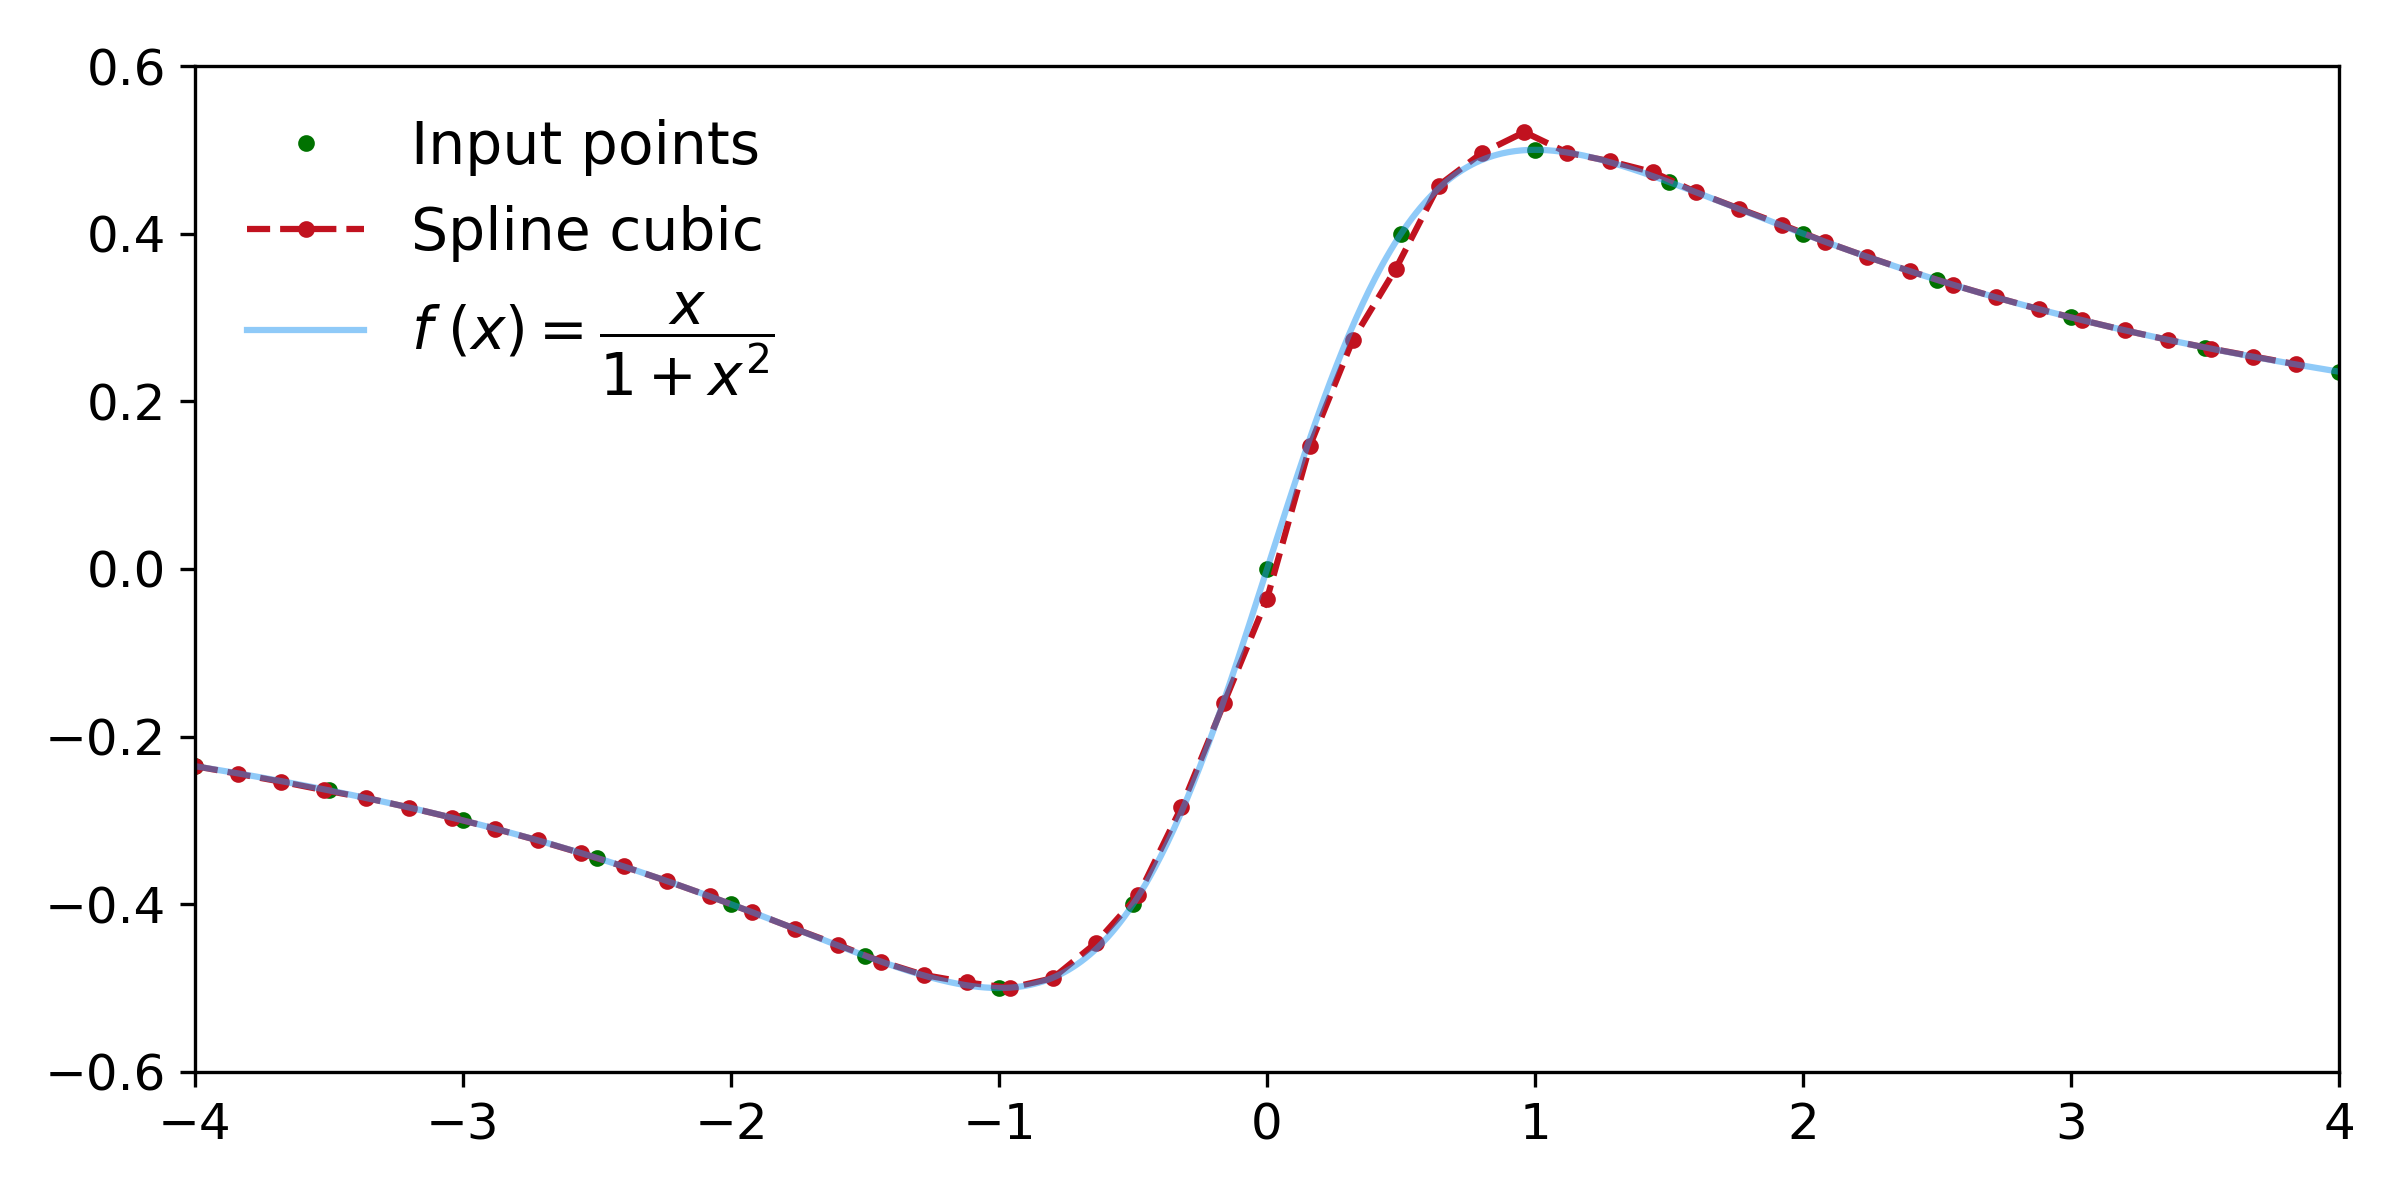
\includegraphics[width=8cm]{Graphics/problema04a_17.png}
		\caption{$n=17$.}
		\label{fig:problema4a_17}
	\end{subfigure}
	\begin{subfigure}[b]{8cm}
		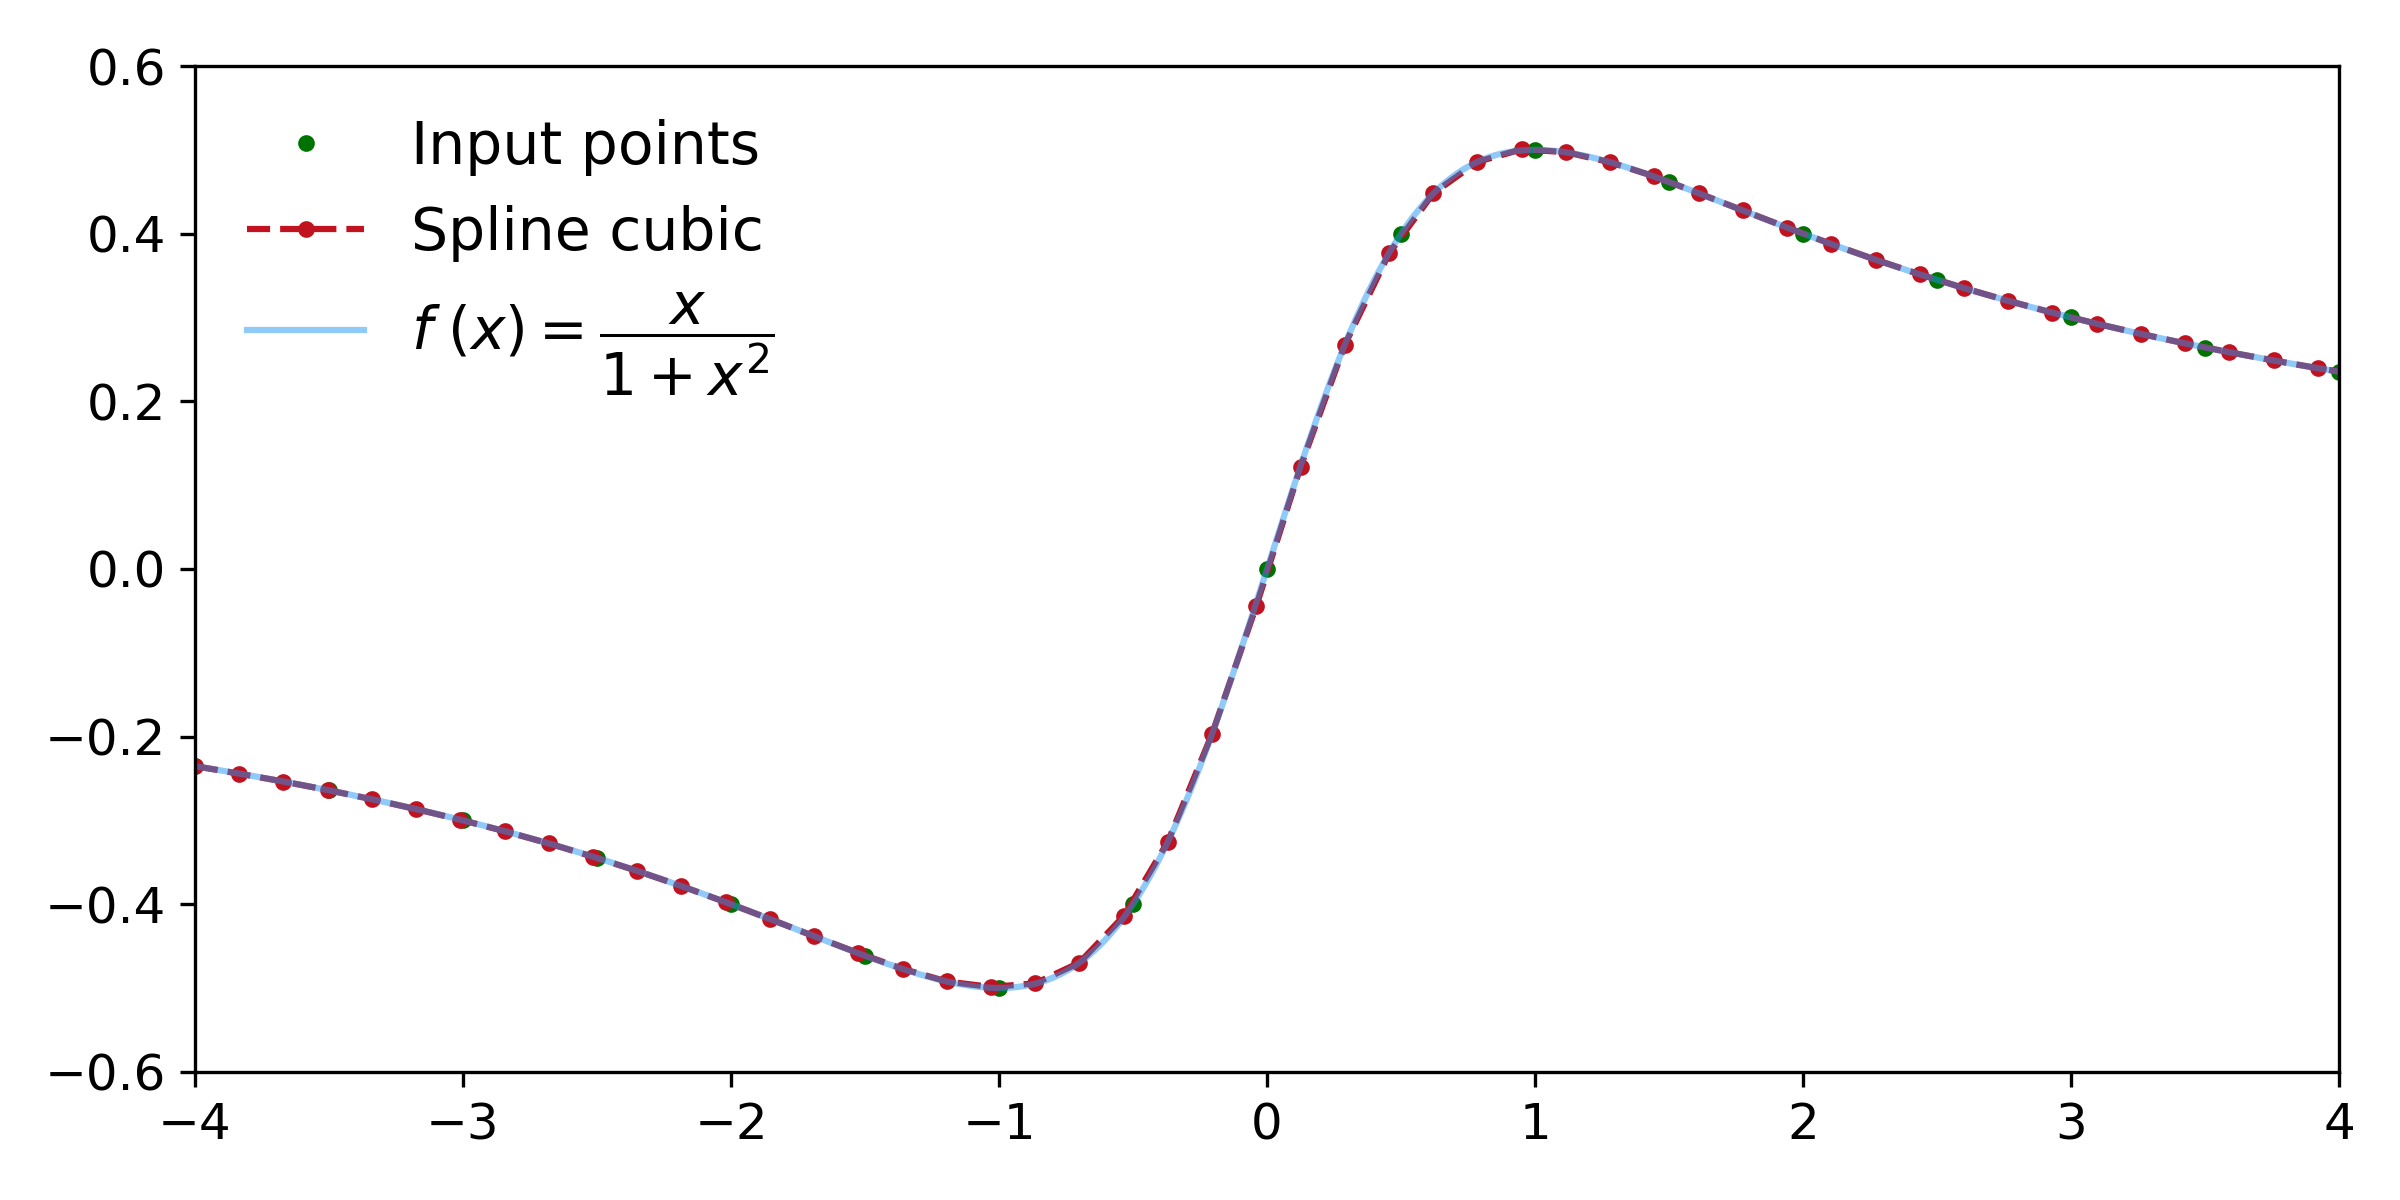
\includegraphics[width=8cm]{Graphics/problema04a_34.png}
		\caption{$n=34$.}
		\label{fig:problema4a_34}
	\end{subfigure}
	\caption{Interpolación de la ecuación \ref{eq:problema4a} dados los puntos generados con las ecuaciones \ref{eq:y_points} y \ref{eq:x_points_modificada}.}
	\label{fig:problema4a}
\end{figure}

Las diferencias entre las gráficas \ref{fig:problema4a_17} y \ref{fig:problema4a_34} radican en el punto de inflexión superior, esto debido a que en la gráfica \ref{fig:problema4a_17} contiene menos puntos para obtener los parámetros en esa región en comparación a la gráfica \ref{sub@fig:problema4a_34}. A pesar de estas diferencias, la inteprolación obtenida con $n=17$ es aceptable, debido a que las diferencias con la función original son despreciables en la región analizada.